\documentclass{article}

\usepackage[utf8]{inputenc}
\usepackage{graphicx}
\usepackage{titling}
\usepackage{amsmath}
\usepackage{amssymb}
\usepackage{cite}
\usepackage{hyperref}
\usepackage{float}
\usepackage{listings}
\usepackage{xcolor}
\usepackage{geometry}

\geometry{a4paper, margin=1in}


\begin{document}

\definecolor{codegreen}{rgb}{0,0.6,0}
\definecolor{codegray}{rgb}{0.5,0.5,0.5}
\definecolor{codepurple}{rgb}{0.58,0,0.82}
\definecolor{backcolour}{rgb}{0.95,0.95,0.92}

\lstdefinestyle{pythonstyle}{
    backgroundcolor=\color{backcolour},   
    commentstyle=\color{codegreen},
    keywordstyle=\color{magenta},
    numberstyle=\tiny\color{codegray},
    stringstyle=\color{codepurple},
    basicstyle=\ttfamily\footnotesize,
    breakatwhitespace=false,         
    breaklines=true,                 
    captionpos=b,                    
    keepspaces=true,                 
    numbers=left,                    
    numbersep=5pt,                  
    showspaces=false,                
    showstringspaces=false,
    showtabs=false,                  
    tabsize=2
}

\lstset{style=pythonstyle}




% Custom title page
\begin{titlepage}
    \begin{center}
        \begin{minipage}[c]{0.12\textwidth}
            
\includegraphics[width=\textwidth]{Cairo_University_Crest.png}
        \end{minipage}
        \hfill
        \begin{minipage}[c]{0.5\textwidth}
            \centering
            {\large Cairo University - Faculty Of Engineering \\ Computer Engineering Department \\ Communication  - Spring 2025 \par}
        \end{minipage}
        \hfill
        \begin{minipage}[c]{0.15\textwidth}
            
\includegraphics[width=\textwidth]{CUFE.jpeg}
        \end{minipage}
    \end{center}
    
    \noindent\hrulefill
    
    \vspace{2cm}
    
    \begin{center}
        {\Huge \textbf{Digital Communications: Assignment 1 (Quantization)}\par}
        \vspace{1.5cm}
        {\Large \textbf{Akram Hany}\par}
        {\Large \textbf{Amir Kedis (9220166)}\par}
        \vspace{1cm}
        {\large Spring 2025\par}
    \end{center}
    
    \vfill
    
\end{titlepage}

\section{Introduction}

In this report, we provide our solution / implementation for Quantization. Covering concepts like midtread and midrise, SNR, uniform and non-uniform quantizers.

\section{Theoretical Background}

\subsection{Uniform Quantization}

Uniform quantization is a process where the input signal amplitude range is divided into equal intervals. The key parameters in uniform quantization are:

\begin{itemize}
    \item Number of levels: $L = 2^n$ where $n$ is the number of bits
    \item Level amplitude: $\Delta = \frac{A_{max} - A_{min}}{L}$
    \item Quantization step size: $\Delta = \frac{2A_m}{L}$ where $A_m$ is the maximum amplitude
    \item Quantization error: $q = \frac{\Delta}{2}$
\end{itemize}

The quantization error is bounded by: $-\frac{\Delta}{2} < q \leq \frac{\Delta}{2}$

\subsection{Signal-to-Noise Ratio (SNR)}

For uniform quantization, the theoretical SNR can be calculated as:

$$SNR_{avg} = \frac{3\alpha^2 L^2}{\Delta^2/12} = 3\alpha^2 2^{2n}$$

Where $\alpha$ is a signal-dependent parameter. In decibels:

$$SNR_{Peak} = 10\log_{10}(3\alpha^2) + 6n$$

For a full-scale sinusoidal input:

$$SNR_{Peak} = 10\log_{10}(3) + 6n$$

\subsection{Midtread and Midrise Quantizers}

Two common types of uniform quantizers are midtread and midrise:

\begin{itemize}
    \item \textbf{Midtread Quantizer}: Has voltage levels centered on integer values, including zero
    \item \textbf{Midrise Quantizer}: Has voltage levels centered on half-integer values, without a level at zero
\end{itemize}

\subsection{Non-uniform Quantization}

For non-uniform signals in uniform quantizers, the SNR performance degrades. To improve performance, non-uniform quantization through companding can be used, with the SQNR given by:

$$SQNR_{non-uniform} = \frac{3L^2}{\ln^2(1+\mu)}$$

Where $\mu$ is the compression parameter.

\section{Methodology}

Our analysis involves implementing both uniform and non-uniform quantization techniques and evaluating their performance through:

\begin{enumerate}
    \item Implementation of midtread and midrise quantizers
    \item Comparison of computational results with theoretical calculations
    \item Analysis of SNR performance across different bit depths
    \item Evaluation of companding effects on non-uniform signals
\end{enumerate}

\section{Results and Discussion}

\subsection{Midtread and Midrise Quantization}

\begin{figure}[H]
    \centering
    \includegraphics[width=0.8\textwidth]{figure1.png}
    \caption{Original signal and its quantized version using midtread (m=1) and midrise (m=0) quantizers}
    \label{fig:midtread_midrise}
\end{figure}

Figure \ref{fig:midtread_midrise} shows the original signal and its quantized version using both midtread (m=1) and midrise (m=0) quantizers. The midtread quantizer includes a level at zero, while the midrise quantizer has levels at half-integer values.

\begin{figure}[H]
    \centering
    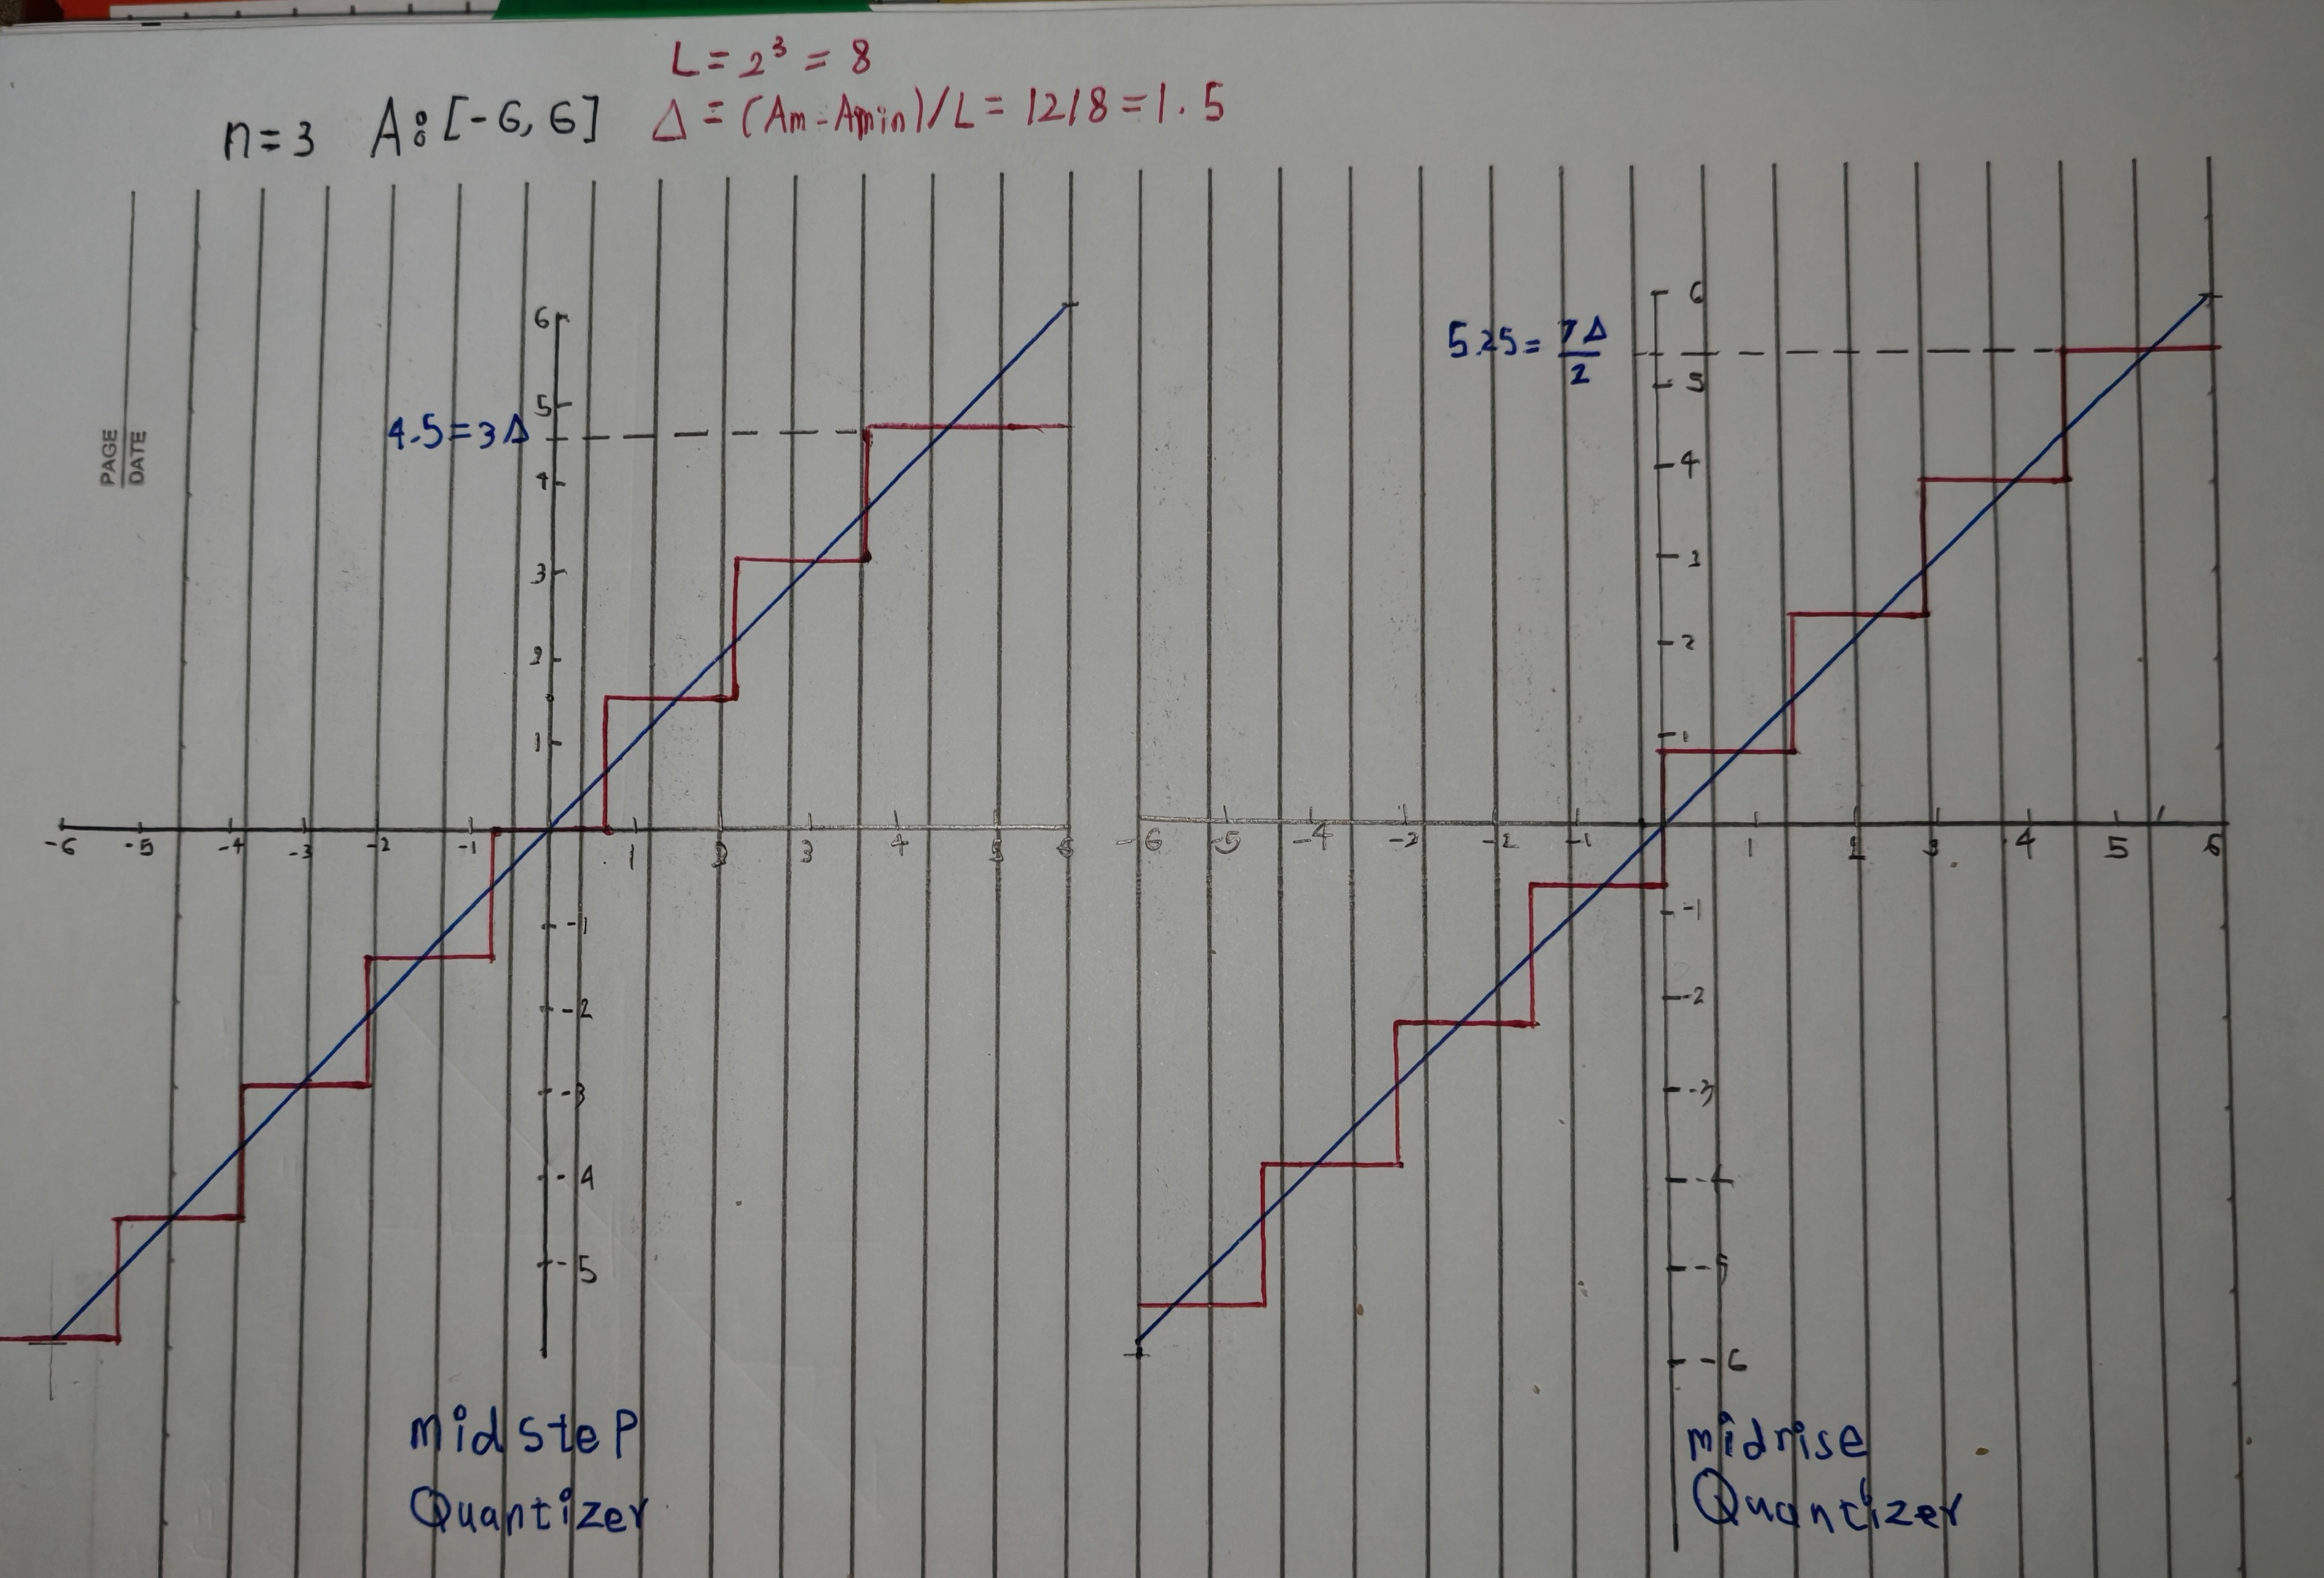
\includegraphics[width=0.8\textwidth]{figure-2.jpg}
    \caption{Manual calculation and hand-drawing of quantization processes for verification}
    \label{fig:manual_calc}
\end{figure}

Figure \ref{fig:manual_calc} presents a manual calculation and hand drawing of the same quantization processes to verify the results.

\subsection{SNR Analysis}

\begin{figure}[H]
    \centering
    \includegraphics[width=0.8\textwidth]{figure3.png}
    \caption{SNR across different bit depths (n) - Linear scale}
    \label{fig:snr_linear}
\end{figure}

Figure \ref{fig:snr_linear} displays the SNR across different bit depths (n) for both theoretical and calculated values in linear scale. As expected, the SNR increases linearly with the number of bits.

\begin{figure}[H]
    \centering
    \includegraphics[width=0.8\textwidth]{figure4.png}
    \caption{SNR across different bit depths (n) - Decibel scale}
    \label{fig:snr_db}
\end{figure}

Figure \ref{fig:snr_db} presents the same data in decibel scale, showing the expected 6 dB improvement in SNR for each additional bit of quantization.

\begin{figure}[H]
    \centering
    \includegraphics[width=0.8\textwidth]{figure5.png}
    \caption{SNR for non-uniform signals in uniform quantizers - Linear scale}
    \label{fig:nonuniform_linear}
\end{figure}

\begin{figure}[H]
    \centering
    \includegraphics[width=0.8\textwidth]{figure6.png}
    \caption{SNR for non-uniform signals in uniform quantizers - Decibel scale}
    \label{fig:nonuniform_db}
\end{figure}

Figures \ref{fig:nonuniform_linear} and \ref{fig:nonuniform_db} show the SNR performance for non-uniform signals processed through uniform quantizers, highlighting the degradation in performance compared to uniform signals.

\subsection{Companding Analysis}

\begin{figure}[H]
    \centering
    \includegraphics[width=0.8\textwidth]{figure7.png}
    \caption{Effect of compression parameter ($\mu$) on SNR performance}
    \label{fig:companding}
\end{figure}

Figure \ref{fig:companding} illustrates the effect of different compression parameters ($\mu$) on the SNR performance of the compander-expander system, demonstrating how appropriate selection of $\mu$ can optimize performance for specific signal distributions.

\section{Conclusion}

Our analysis confirms the theoretical expectations regarding quantization performance:

\begin{enumerate}
    \item The SNR improves by approximately 6 dB for each additional bit in the quantizer
    \item Midtread and midrise quantizers show different characteristics, particularly in how they handle signals near zero
    \item Non-uniform signals experience degraded performance in uniform quantizers
    \item Companding can significantly improve performance for non-uniform signals when the compression parameter is properly selected
\end{enumerate}

These findings highlight the importance of selecting appropriate quantization techniques based on the specific characteristics of the input signal in digital communication systems.

\appendix

\section{Python Implementation}

\label{appendix:code}

This appendix contains the Python code used to implement the quantization techniques and generate the figures presented in this report.

\subsection{Uniform Quantization Implementation}

\begin{lstlisting}[language=Python, caption=Uniform Quantization Implementation]
plt.show()
\end{lstlisting}

\subsection{SNR Analysis Implementation}

\begin{lstlisting}[language=Python, caption=SNR Analysis Implementation]
plt.show()
\end{lstlisting}

\subsection{Non-uniform Quantization Implementation}

\begin{lstlisting}[language=Python, caption=Non-uniform Quantization and Companding Implementation]

plt.show()
\end{lstlisting}


\end{document}